

\documentclass[journal,12pt,twocolumn]{IEEEtran}

\usepackage{setspace}
\usepackage{gensymb}
\usepackage{caption}
\usepackage[parfill]{parskip}
\singlespacing

\usepackage[cmex10]{amsmath}
\usepackage{amsthm}
\usepackage{mathrsfs}
\usepackage{txfonts}
\usepackage{stfloats}
\usepackage{cite}
\usepackage{cases}
\usepackage{subfig}

\usepackage{longtable}
\usepackage{multirow}
\usepackage{enumitem}
\usepackage{mathtools}
\usepackage{tikz}
\usepackage{circuitikz}
\usepackage{verbatim}
\usepackage{hyperref}
\usepackage{tkz-euclide} % loads  TikZ and tkz-base
\usepackage{listings}
    \usepackage{color}                                            %%
    \usepackage{array}                                            %%
    \usepackage{longtable}                                        %%
    \usepackage{calc}                                             %%
    \usepackage{multirow}                                         %%
    \usepackage{hhline}                                           %%
    \usepackage{ifthen}                                           %%
    \usepackage{lscape}     
\usepackage{multicol}
\usepackage{chngcntr}
\usepackage{iftex}
\usepackage{geometry}
\usepackage{bm}
\usepackage{array}
\newcolumntype{L}[1]{>{\raggedright\let\newline\\\arraybackslash\hspace{0pt}}m{#1}}
\newcolumntype{C}[1]{>{\centering\let\newline\\\arraybackslash\hspace{0pt}}m{#1}}
\newcolumntype{R}[1]{>{\raggedleft\let\newline\\\arraybackslash\hspace{0pt}}m{#1}}
\def \hsp {\hspace{3mm}}

\makeatletter

\providecommand{\tabularnewline}{\\}



\makeatother
\ifxetex
\usepackage[T1]{fontenc}
\usepackage{fontspec}

\newfontfamily\nakulafont[Script=Devanagari,AutoFakeBold=2,Path = fonts/]{Nakula}
\fi
\usepackage{tikz}
\usepackage{xcolor}
\DeclareMathOperator*{\Res}{Res}
\DeclareMathOperator*{\pipe}{|}
\renewcommand\thesection{\arabic{section}}
\renewcommand\thesubsection{\thesection.\arabic{subsection}}
\renewcommand\thesubsubsection{\thesubsection.\arabic{subsubsection}}

\renewcommand\thesectiondis{\arabic{section}}
\renewcommand\thesubsectiondis{\thesectiondis.\arabic{subsection}}
\renewcommand\thesubsubsectiondis{\thesubsectiondis.\arabic{subsubsection}}

% correct bad hyphenation here
\hyphenation{op-tical net-works semi-conduc-tor}
\def\inputGnumericTable{}                                 %%

\lstset{
language=tex,
frame=single, 
breaklines=true
}

\newtheorem{theorem}{Theorem}[section]
\newtheorem{problem}{Problem}
\newtheorem{proposition}{Proposition}[section]
\newtheorem{lemma}{Lemma}[section]
\newtheorem{corollary}[theorem]{Corollary}
\newtheorem{example}{Example}[section]
\newtheorem{definition}[problem]{Definition}
\newcommand{\BEQA}{\begin{eqnarray}}
\newcommand{\EEQA}{\end{eqnarray}}
\newcommand{\define}{\stackrel{\triangle}{=}}

\bibliographystyle{IEEEtran}



\providecommand{\mbf}{\mathbf}
\providecommand{\pr}[1]{\ensuremath{\Pr\left(#1\right)}}
\providecommand{\qfunc}[1]{\ensuremath{Q\left(#1\right)}}
\providecommand{\sbrak}[1]{\ensuremath{{}\left[#1\right]}}
\providecommand{\lsbrak}[1]{\ensuremath{{}\left[#1\right.}}
\providecommand{\rsbrak}[1]{\ensuremath{{}\left.#1\right]}}
\providecommand{\brak}[1]{\ensuremath{\left(#1\right)}}
\providecommand{\lbrak}[1]{\ensuremath{\left(#1\right.}}
\providecommand{\rbrak}[1]{\ensuremath{\left.#1\right)}}
\providecommand{\cbrak}[1]{\ensuremath{\left\{#1\right\}}}
\providecommand{\lcbrak}[1]{\ensuremath{\left\{#1\right.}}
\providecommand{\rcbrak}[1]{\ensuremath{\left.#1\right\}}}
\theoremstyle{remark}
\newtheorem{rem}{Remark}
\newcommand{\sgn}{\mathop{\mathrm{sgn}}}
\providecommand{\abs}[1]{\left\vert#1\right\vert}
\providecommand{\res}[1]{\Res\displaylimits_{#1}} 
\providecommand{\norm}[1]{\left\lVert#1\right\rVert}
%\providecommand{\norm}[1]{\lVert#1\rVert}
\providecommand{\mtx}[1]{\mathbf{#1}}
\providecommand{\mean}[1]{E\left[ #1 \right]}
\providecommand{\fourier}{\overset{\mathcal{F}}{ \rightleftharpoons}}
\providecommand{\system}[1]{\overset{\mathcal{#1}}{ \longleftrightarrow}}
\providecommand{\gauss}[2]{\mathcal{N}\ensuremath{\left(#1,#2\right)}}
%
	%\newcommand{\solution}[2]{\textbf{Solution:}{#1}}
\newcommand{\solution}{\noindent \textbf{Solution: }}
\newcommand{\cosec}{\,\text{cosec}\,}
\newcommand{\sinc}{\,\text{sinc}\,}
\newcommand{\rect}{\,\text{rect}\,}
\providecommand{\dec}[2]{\ensuremath{\overset{#1}{\underset{#2}{\gtrless}}}}
\newcommand{\myvec}[1]{\begin{pmatrix}#1\end{pmatrix}}
\newcommand{\mydet}[1]{\ensuremath{\begin{vmatrix}#1\end{vmatrix}}}
\newcommand*{\permcomb}[4][0mu]{{{}^{#3}\mkern#1#2_{#4}}}
\newcommand*{\perm}[1][-3mu]{\permcomb[#1]{P}}
\newcommand*{\comb}[1][-1mu]{\permcomb[#1]{C}}
%\numberwithin{equation}{section}
\numberwithin{equation}{section}
% \numberwithin{figure}{section}
%\numberwithin{definition}{section}
% \makeatletter
% \@addtoreset{figure}{problem}
% \makeatother

\let\StandardTheFigure\thefigure
\let\vec\mathbf
\renewcommand{\thefigure}{\arabic{figure}}
%\renewcommand{\thefigure}{\theproblem}
\vspace{3cm}
\numberwithin{equation}{section}



%\usepackage{babel}

\graphicspath{{../images/}}
\begin{document}

    \title{Probability Distributions}
    \author{Abhay Shankar K : cs21btech11001}
    
    \newcommand{\e}[1]{\ensuremath{e^{#1}}}
	\providecommand{\pdf}[2]{\ensuremath{p_{#2}\left(#1\right)}}
	\providecommand{\cdf}[2]{\ensuremath{P_{#2}\left(#1\right)}}
    \providecommand{\inv}[1]{\ensuremath{\frac{1}{#1}}}
    \providecommand{\der}[4]{\ensuremath{\frac{#3 #1}{#4 #2}}}
    \providecommand{\oder}[2]{\der{#1}{#2}{d}{d}}
    \providecommand{\pder}[2]{\der{#1}{#2}{\partial}{\partial}}
\maketitle
\tableofcontents
\listoffigures

\newpage

\section{Uniform Random Numbers}

Let $U$ be a uniform random variable between 0 and 1.

\begin{enumerate}[label=\thesection.\arabic*,ref=\thesection.\theenumi]
\item Generate $10^6$ samples of $U$ using a C program and save into a file called uni.dat.

\solution Download the following files and execute the C program.

\begin{lstlisting}
wget https://github.com/Abhay478/GVV_things/blob/master/code/coeffs.h
wget https://github.com/Abhay478/GVV_things/blob/master/code/exrand.c
\end{lstlisting}
    
    \begin{lstlisting}
gcc exrand.c -o exrand && ./exrand
    \end{lstlisting}

Or download the sample file
\begin{lstlisting}
wget https://github.com/Abhay478/GVV_things/blob/master/data/uni.dat   
\end{lstlisting}

%
\item
Load the uni.dat file into python and plot the empirical CDF of $U$ using the samples in uni.dat. The CDF is defined as
\begin{align}
    \cdf{x}{U} = \pr{U \le x}
\end{align}

\solution  

The following code plots the figure \ref{fig:uni_cdf}
\begin{lstlisting}
wget https://github.com/Abhay478/GVV_things/blob/master/code/cdf_plot_unif.py
\end{lstlisting}

\begin{lstlisting}
python3 cdf_plot_unif.py
\end{lstlisting}

\begin{figure}[!h]
    \centering
    \caption{The CDF of $U$}
    \includegraphics[width=\columnwidth]{unif.png}
        \label{fig:uni_cdf}
\end{figure}

%
\item
Find a  theoretical expression for $\cdf{x}{U}$.

\solution
We know that 
\begin{equation}
    \cdf{x}{U} = \int_{-\infty}^\infty \pdf{x}{U}
\end{equation}

Therefore,
		\begin{align}
			\cdf{x}{U} &= \int_{-\infty}^\infty U(x) dx \nonumber \\
			&= \int_{-\infty}^\infty u(x) - u(x - 1) dx \nonumber \\
			\therefore \cdf{x}{U} &= 
			\begin{cases}
				0\ \forall x < 0 \\
				x\ \forall x \in [0, 1] \\
				1\ \forall x > 1
			\end{cases}
                \label{uni-cdf}
		\end{align}

		Here, $u(x)$ is the step function.

\item
The mean of $U$ is defined as
%
\begin{equation}
E\sbrak{U} = \inv{N}\sum_{i=1}^{N}U_i
\end{equation}
%
and its variance as
%
\begin{equation}
\text{var}\sbrak{U} = E\sbrak{U- E\sbrak{U}}^2 
\end{equation}

Write a C program to  find the mean and variance of $U$.

\solution

\begin{lstlisting}
wget https://github.com/Abhay478/GVV_things/blob/master/code/mean-var.c
\end{lstlisting}

\begin{lstlisting}
gcc mean-var.c -o mean-var && ./mean-var
\end{lstlisting}


\item Verify your result theoretically given that
\end{enumerate}
%
\begin{equation}
E\sbrak{U^k} = \int_{-\infty}^{\infty}x^kdF_{U}(x)
\end{equation}

\solution

The mean, $E[U]$,

\begin{align}
    E[U] &= \int_{-\infty}^\infty x U(x) dx \nonumber \\
    &= \int_0^1 x dx \nonumber \\
    &= 0.5
\end{align}

The experimental result was $0.500$.

The variance, $Var[U] = E[U^2] - E^2[U]$,
\begin{align}
    E[U^2] &= \int_{-\infty}^\infty x^2 U(x) dx \nonumber \\
    &= \int_0^1 x^2 dx \nonumber \\
    &= \frac{1}{3} \\
    \therefore Var[U] &= \frac{1}{3} - \brak{\frac{1}{2}}^2 \nonumber \\
    &= \frac{1}{12}
\end{align}

The experimental result was $0.083$.

\newpage

\section{Central Limit Theorem}
%
\begin{enumerate}[label=\thesection.\arabic*,ref=\thesection.\theenumi]

%
\item
Generate $10^6$ samples of the random variable
%
\begin{equation}
X = \sum_{i=1}^{12}U_i -6
\end{equation}
%
using a C program, where $U_i, i = 1,2,\dots, 12$ are  a set of independent uniform random variables 
between 0 and 1 and save in a file called gau.dat

\solution

% \begin{lstlisting}
% wget https://github.com/Abhay478/GVV_things/blob/master/code/coeffs.h
% wget https://github.com/Abhay478/GVV_things/blob/master/code/exrand.c
% \end{lstlisting}
        
    \begin{lstlisting}
gcc exrand.c -o exrand && ./exrand
    \end{lstlisting}

    Or downlload the sample file.
    \begin{lstlisting}
wget https://github.com/Abhay478/GVV_things/blob/master/data/gau.dat
    \end{lstlisting}

\item
Load gau.dat in python and plot the empirical CDF of $X$ using the samples in gau.dat. 
What properties does a CDF have?

\solution 

\begin{itemize}
    \item All CDFs are monotonically increasing
    \item All CDFs are continuous over their domain
    \item $\lim_{n \rightarrow \infty} \cdf{x}{X} = 1$
    \item $\lim_{n \rightarrow -\infty} \cdf{x}{X} = 0$
\end{itemize}

The CDF of $X$ is plotted below.

.
\begin{lstlisting}
wget https://github.com/Abhay478/GVV_things/blob/master/code/cdf_plot_gau.py
\end{lstlisting}

\begin{lstlisting}
python3 cdf_plot_gau.py
\end{lstlisting}

\begin{figure}[!h]
    \caption{The CDF of $X$}
    \includegraphics[width=\columnwidth]{gau.png}
\end{figure}

\item

Load gau.dat in python and plot the empirical PDF of $X$ using the samples in gau.dat. The PDF of $X$ is defined as
\begin{align}
\pdf{x}{X} = \frac{d}{dx}\cdf{x}{X}
\end{align}


What properties does the PDF have?

\solution 

Properties of a PDF:

\begin{itemize}
    \item The PDF adheres to unitarity, i.e. its integral over the real line is 1
    \item The PDF is always nonnegative
    \item The PDF is finite at all points
\end{itemize}

\begin{lstlisting}
wget https://github.com/Abhay478/GVV_things/blob/master/code/pdf_plot_gau.py
\end{lstlisting}

\begin{lstlisting}
python3 pdf_plot_gau.py
\end{lstlisting}

\begin{figure}[!h]
\centering
\includegraphics[width=\columnwidth]{pdf_gau.png}
\caption{The PDF of $X$}
\label{fig:gauss_pdf}
\end{figure}

\item Find the mean and variance of $X$ by writing a C program.

\begin{lstlisting}
wget https://github.com/Abhay478/GVV_things/blob/master/code/mean-var.c
\end{lstlisting}

\begin{lstlisting}
gcc mean-var.c -o mean-var && ./mean-var
\end{lstlisting}

\item Given that 
\begin{align}
    \pdf{x}{X} = \frac{1}{\sqrt{2\pi}}\exp\brak{-\frac{x^2}{2}}, -\infty < x < \infty,
\end{align}

repeat the above exercise theoretically.

\solution

Given 
\begin{align}
    \pdf{x}{X} = \inv{\sqrt{2 \pi}} \e{-\frac{x^2}{2}} \label{pdf-gau}
\end{align}

We use the substitution $u = \frac{x^2}{2}$, whence $du = x dx$.

The mean,
\begin{align}
    E[X] &= \int_{-\infty}^\infty \frac{x}{\sqrt{2 \pi}} \e{-\frac{x^2}{2}} dx \nonumber \\
    &= \inv{\sqrt{2 \pi}} \int_{-\infty}^\infty u \e{-u} du \nonumber \\
    &= 0
\end{align}

The variance, $Var[X] = E[X^2]$, since $E[X] = 0$.

\begin{align}
    Var[X] &= \int_{-\infty}^\infty \frac{x^2}{\sqrt{2 \pi}} \e{-\frac{x^2}{2}} dx \nonumber \\
    &= \inv{\sqrt{\pi}} \int_{-\infty}^\infty \sqrt{u} \e{-u} du \\
    &\text{ Which is clearly } 2 \Gamma\brak{\frac{3}{2}} \nonumber \\
    &= \frac{2}{\sqrt{\pi}} \times \frac{\sqrt{\pi}}{2} = 1
\end{align}



\end{enumerate}
\newpage

\section{From Uniform to Other}
\begin{enumerate}[label=\thesection.\arabic*,ref=\thesection.\theenumi]
%
\item
Generate samples of 
%
\begin{equation}
V = -2\ln\brak{1-U}
\end{equation}
%
and plot its CDF.  

% \begin{lstlisting}
% wget https://github.com/Abhay478/GVV_things/blob/master/code/coeffs.h
% wget https://github.com/Abhay478/GVV_things/blob/master/code/exrand.c
% \end{lstlisting}
    
    \begin{lstlisting}
gcc exrand.c -o exrand && ./exrand
    \end{lstlisting}

Or download the sample file
\begin{lstlisting}
wget https://github.com/Abhay478/GVV_things/blob/master/data/exp.dat   
\end{lstlisting}

The following python code plots the CDF.
\begin{lstlisting}
wget https://github.com/Abhay478/GVV_things/blob/master/code/cdf_plot_exp.py
\end{lstlisting}
    
\begin{lstlisting}
python3 cdf_plot_exp.py
\end{lstlisting}

\begin{figure}[!h]
    \caption{CDF of Exponential}
    \includegraphics[width = \columnwidth]{exp.png}
\end{figure}

\item Find a theoretical expression for $F_V(x)$.

\solution

Let
\begin{align}
    v = -2ln(1 - u) \nonumber \\
    \implies u = 1 - \e{-\frac{v}{2}} \label{exp-cdf}
\end{align}

Let
\begin{align}
    f(t) &= -2ln(1 - t) \label{Vfunc} \\
    \implies f'(t) &= \frac{2}{1 - t} \text{ which is increasing}\\
    \therefore Pr(V < v) &= Pr\brak{U < 1 - \e{-\frac{v}{2}}} \nonumber \\
\end{align}

We know that $Pr(U < f(x)) = f(x)$ if $f(x) \leq 1$ 

\begin{align}
    \cdf{x}{V} &= 
    \begin{cases}
        0 \text{ if } x < 0 \\
        1 - \e{-\frac{x}{2}} \text{ if } x \geq 0\\
    \end{cases}
\end{align}


Differentiating,

\begin{align}
    \pdf{x}{V} &= u(x)\frac{\e{-\frac{x}{2}}}{2} \label{exp-pdf}
\end{align}

The PDF is clearly as exponential distribution with $\lambda = 0.5$.
\begin{lstlisting}
wget https://github.com/Abhay478/GVV_things/blob/master/code/pdf_plot_exp.py
\end{lstlisting}
    
\begin{lstlisting}
python3 pdf_plot_exp.py
\end{lstlisting}

\begin{figure}[!h]
    \caption{PDF of Exponential}
    \includegraphics[width = \columnwidth]{pdf_exp.png}
\end{figure}
%
%\item
%Generate the Rayleigh distribution from Uniform. Verify your result through graphical plots.
\end{enumerate}

\newpage

\section{Triangular Distribution}
\begin{enumerate}[label=\thesection.\arabic*,ref=\thesection.\theenumi]

\item Generate 
	\begin{align}
		T = U_1+U_2
	\end{align}
\solution

% \begin{lstlisting}
% wget https://github.com/Abhay478/GVV_things/blob/master/code/coeffs.h
% wget https://github.com/Abhay478/GVV_things/blob/master/code/exrand.c
% \end{lstlisting}
    
    \begin{lstlisting}
gcc exrand.c -o exrand && ./exrand
    \end{lstlisting}

Or download the sample file
\begin{lstlisting}
wget https://github.com/Abhay478/GVV_things/blob/master/data/tri.dat   
\end{lstlisting}

\item Find the CDF of $T$.

\solution

\begin{lstlisting}
wget https://github.com/Abhay478/GVV_things/blob/master/code/cdf_plot_tri.py
\end{lstlisting}

\begin{lstlisting}
python3 cdf_plot_tri.py
\end{lstlisting}

\item Find the PDF of $T$.

\solution 

\begin{lstlisting}
wget https://github.com/Abhay478/GVV_things/blob/master/code/pdf_plot_tri.py
\end{lstlisting}

\begin{lstlisting}
python3 pdf_plot_tri.py
\end{lstlisting}

\item Find the theoretical expressions for the PDF and CDF of $T$.

\solution
The CDF:
\begin{align}
    \cdf{t}{T} &= \int_{-\infty}^\infty \cdf{t - u}{U_1} \pdf{u}{U_2} du \nonumber \\
    &= \int_{t - 1}^t dx \begin{cases}
        0\ \forall x < 0 \\
				x\ \forall x \in [0, 1] \\
				1\ \forall x > 1
    \end{cases} \\
&= \begin{cases}
    0\ \forall t < 0 \\
    \frac{t^2}{2}\ \forall t \in \sbrak{0, 1} \\
    2t - \frac{t^2}{2} - 1\ \forall t \in \sbrak{1, 2} \\
    1\ \forall t > 2
\end{cases} \label{tri-cdf}
\end{align}

Differentiating the equation $~\eqref{tri-cdf}$, 
\begin{align}
    \pdf{t}{T} = \begin{cases}
        1 - \abs{1 - t} \ \forall t \in \sbrak{0, 2} \\
        0\ otherwise
    \end{cases} \label{tri-pdf}
\end{align}

\newpage
\item Verify your results through a plot. 
\begin{figure}[!h]
    \caption{CDF of Triangular}
    \includegraphics[width = \columnwidth]{tri.png}
\end{figure}

\begin{figure}[!h]
    \caption{PDF of Triangular}
    \includegraphics[width = \columnwidth]{pdf_tri.png}
\end{figure}

\end{enumerate}

\newpage

\section{Maximum Likelihood}
\begin{enumerate}[label=\thesection.\arabic*, ref=\thesection.\theenumi]
\item Generate equiprobable $X \in \cbrak{1,-1}$.

% \begin{lstlisting}
% wget https://github.com/Abhay478/GVV_things/blob/master/code/coeffs.h
% wget https://github.com/Abhay478/GVV_things/blob/master/code/exrand.c
% \end{lstlisting}
        
    \begin{lstlisting}
gcc exrand.c -o exrand && ./exrand
    \end{lstlisting}

    Or download the sample files.
\begin{lstlisting}
wget https://github.com/Abhay478/GVV_things/blob/master/data/plm.dat
\end{lstlisting}
\item Generate 
\begin{equation}
Y = AX+N,
\end{equation}
		where $A = 5$ dB,  and $N \sim \gauss{0}{1}$.

Or download the sample files
\begin{lstlisting}
wget https://github.com/Abhay478/GVV_things/blob/master/data/noi.dat
\end{lstlisting}
    
	\item Plot $Y$ using a scatter plot.
	
	\solution

    \begin{lstlisting}
wget https://github.com/Abhay478/GVV_things/blob/master/code/scatter.py
    \end{lstlisting}

    \begin{lstlisting}
python3 scatter.py
    \end{lstlisting}
	
    \begin{figure}[!h]
        \caption{Scatterplot}
        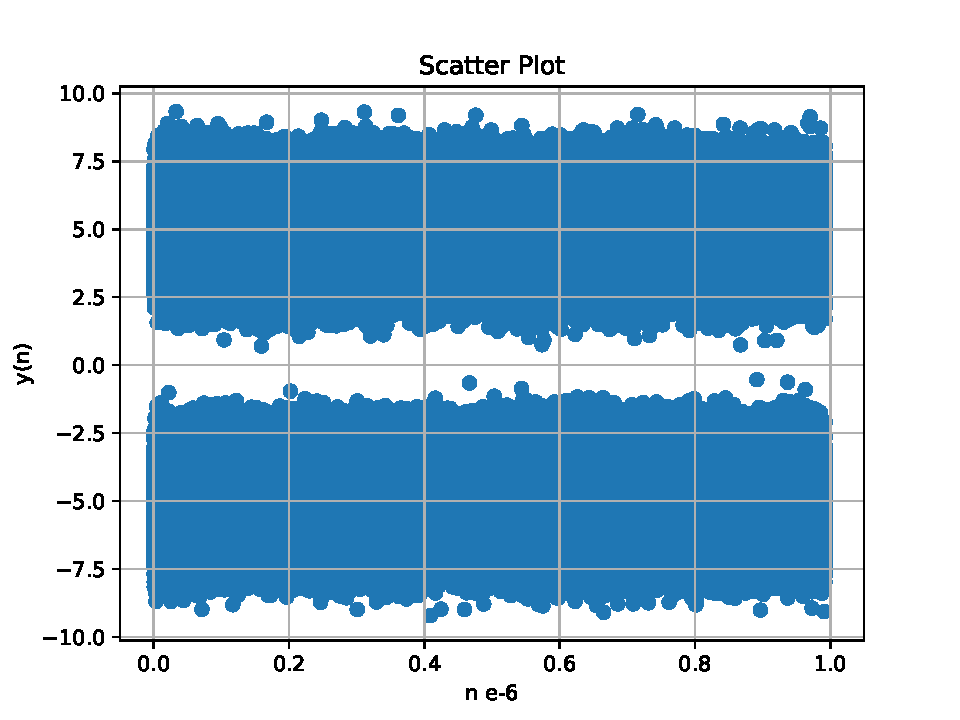
\includegraphics[width = \columnwidth]{scat.png} 
    \end{figure}

	\item Guess how to estimate $X$ from $Y$.

	\solution

	From the scatter plot, it is evident that $Y > 0$ usually correlates to $X = 1$, and 
    $Y < 0$ to $X = -1$
\item
\label{ml-ch4_sim}
Find 
\begin{equation}
	P_{e \pipe 0} = \pr{\hat{X} = -1 \pipe X=1}
\end{equation}
and 
\begin{equation}
	P_{e \pipe 1} = \pr{\hat{X} = 1 \pipe X=-1}
\end{equation}

\solution

The following code prints the number of samples that are incorrectly 
estimated. It is zero.

It also prints the theoretical value, which is an order of 
magnitude too small for our sample size. 

\begin{lstlisting}
wget https://github.com/Abhay478/GVV_things/blob/master/code/estim.py
\end{lstlisting}

\begin{lstlisting}
python3 estim.py
\end{lstlisting}

Therefore, according to the simulation, 

\begin{equation}
	P_{e\pipe0} = 0
\end{equation}
and 
\begin{equation}
	P_{e\pipe1} = 0
\end{equation}

\item Find $P_e$ assuming that $X$ has equiprobable symbols.

\begin{align}
    P_{e\pipe0} &= \pr{\hat{X} = -1 \pipe X=1}  \label{P-e-def} \\
    &= \pr{Y < 0 \pipe X = 1} \nonumber \\
    &= \pr{N < -A} \nonumber \\
    &= \mathbf{Q}\brak{A}
\end{align}

Similarly, due to the symmetry of the gaussian, $P_{e\pipe1} = \mathbf{Q}\brak{A}$.

With $A = 5 dB$,
\begin{equation}
	P_{e\pipe0} = \mathbf{Q}\brak{5}
\end{equation}
and 
\begin{equation}
	P_{e\pipe1} = \mathbf{Q}\brak{5}
\end{equation}
where
\begin{equation}
    \mathbf{Q}\brak{5} = 2.866 \cdot 10^{-7}
\end{equation}

\item
Verify by plotting  the theoretical $P_e$ with respect to $A$ from 0 to 10 dB.  

\begin{lstlisting}
wget https://github.com/Abhay478/GVV_things/blob/master/code/Q_func.py
\end{lstlisting}

\begin{lstlisting}
python3 Q_func.py
\end{lstlisting}

\begin{figure}[!h]
    \caption{Q function}
    \includegraphics[width = \columnwidth]{Q.png}
\end{figure}

\begin{figure}[!h]
    \includegraphics[width = \columnwidth]{Q_log.png}
\end{figure}

\item Now, consider a threshold $\delta$  while estimating $X$ from $Y$. Find the value of $\delta$ that minimizes the theoretical $P_e$.

Considering the estimation threshold to be $\delta$, we have
\begin{align}
    P_e &= \pdf{-1}{X} \cdf{A + \delta}{N} \nonumber \\
    &+      \pdf{1}{X} \cdf{A - \delta}{N} \label{P-e} \\
    &= \frac{\cdf{A + \delta}{N} + \cdf{A - \delta}{N}}{2} \label{equi-Q}
\end{align}

Differentiating wrt $\delta$ and setting it to zero, we have:
\begin{align}
    \oder{P_e}{\delta} &= \frac{\pdf{A - \delta}{N} - \pdf{A + \delta}{N}}{2}\nonumber \\
    \implies \delta &= 0 \sbrak{\forall A \neq 0}
\end{align}
Differentiating again,
\begin{align}
    \frac{d^2 P_e}{d \delta^2} = \frac{(A - \delta)\e{-\frac{(A - \delta)^2}{2}} + (A + \delta)\e{-\frac{(A + \delta)^2}{2}}}{2\sqrt{2 \pi}}
\end{align}
which is clearly positive for the given parameters, ensuring that $P_e$ is minimized.

\item Repeat the above exercise when 
	\begin{align}
		p_{X}(0) = p
	\end{align}

    From ~\eqref{P-e},
    \begin{align}
        p \pdf{A - \delta}{N} &= (1 - p) \pdf{A + \delta}{N} \nonumber \\
        \implies \e{2A \delta} &= \frac{1 - p}{p} \nonumber \\
        \implies \delta &= \frac{1}{2A} \ln\brak{\frac{1 - p}{p}}
    \end{align}


    \item Repeat the above exercise using the MAP criterion.

    Using Bayes' theorem,
        \begin{align}
            &P(X = 1 \pipe Y = y) = \nonumber \\
            &\frac{P(N = y - A)\cdf{1}{X}}{\cdf{y}{Y}} \nonumber \\
            &= \frac{p\pdf{y - A}{N}}{p\pdf{y - A}{N} + (1 - p)\pdf{y + A}{N}} \nonumber \\
            &= \frac{p}{p + (1 - p)\e{-2yA}}
        \end{align}

    Due to unitarity,
        \begin{align}
            P(X = -1 \pipe Y = y) &= \frac{1 - p}{(1 - p) + p\e{2yA}}
        \end{align}

    Hence, 
% \begin{align}
% 	P_{e \pipe 1} &= \frac{p}{p + \brak{1 - p}\e{-2yA}} \nonumber \\&\stackrel{0}{\stackrel{\gtrless}{1}} \nonumber \\P_{e\pipe0} &= \frac{1 - p}{\brak{1 - p} + pe^{2yA}} \nonumber\\
% 	\implies \frac{(1 - p)^2}{p^2} &\stackrel{0}{\stackrel{\gtrless}{1}} \e{4yA} \nonumber\\
% 	\implies y &\stackrel{0}{\stackrel{\gtrless}{1}} \frac{1}{2A}\ln{\brak{\frac{1 - p}{p}}} \label{threshold}
% \end{align}

\textbf{If $X = 1$}
\begin{align}
        \frac{p}{p + \brak{1 - p}\e{-2yA}} &> \frac{1 - p}{\brak{1 - p} + pe^{2yA}} \nonumber \\
        \implies \frac{(1 - p)^2}{p^2} &> \e{4yA} \nonumber\\
        \implies y &> \frac{1}{2A}\ln{\brak{\frac{1 - p}{p}}} \label{threshold_1}
\end{align}

\textbf{If $X = -1$}
\begin{align}
        \frac{p}{p + \brak{1 - p}\e{-2yA}} &< \frac{1 - p}{\brak{1 - p} + pe^{2yA}} \nonumber \\
        \implies \frac{(1 - p)^2}{p^2} &< \e{4yA} \nonumber\\
        \implies y &< \frac{1}{2A}\ln{\brak{\frac{1 - p}{p}}} \label{threshold_1}
\end{align}

\end{enumerate}

        \newpage

\section{Gaussian to Other}

\begin{enumerate}[label=\thesection.\arabic*,ref=\thesection.\theenumi]
\item
Let $X_1 \sim  \gauss{0}{1}$ and $X_2 \sim  \gauss{0}{1}$. Plot the CDF and PDF of
%
\begin{equation}
V = X_1^2 + X_2^2 
\end{equation}

% \begin{lstlisting}
% wget https://github.com/Abhay478/GVV_things/blob/master/code/coeffs.h
% wget https://github.com/Abhay478/GVV_things/blob/master/code/exrand.c
% \end{lstlisting}
    
    \begin{lstlisting}
gcc exrand.c -o exrand && ./exrand
    \end{lstlisting}

Or download the sample file
\begin{lstlisting}
wget https://github.com/Abhay478/GVV_things/blob/master/data/gss.dat   
\end{lstlisting}

\begin{figure}[!h]
    \caption{CDF of Exponential \(again\)}
    \includegraphics[width = \columnwidth]{gss.png}
\end{figure}

\begin{figure}[!h]
    \caption{PDF of Exponential \(again\)}
    \includegraphics[width = \columnwidth]{pdf_gss.png}
\end{figure}


\item
If
%
\begin{equation}
\cdf{x}{V} = 
\begin{cases}
1 - e^{-\alpha x} & x \geq 0 \\
0 & x < 0,
\end{cases}
\end{equation}
%
find $\alpha$.

\solution

Making standard trigonometric substitutions :
\begin{itemize}
    \item $X_1 = R \cos\brak{\Theta}$
    \item $X_2 = R\sin\brak{\Theta}$
\end{itemize}

Within the domains
\begin{itemize}
    \item $R \in \mathbb{R^+}$
    \item $\Theta \in \sbrak{-\pi, \pi}$
\end{itemize}

Hence, the Jacobian.

\begin{align}
    \mathbb{J} &= \myvec{\pder{X_1}{R} & \pder{X_2}{R} \\ && \\ \pder{X_1}{\Theta} & \pder{X_2}{\Theta}} \nonumber \\
    &= \myvec{\cos\Theta & \sin\Theta \\ -R\sin\Theta & R\cos\Theta} \\
    \implies \abs{\mathbb{J}} &= R
\end{align}

Whence
\begin{align}
    \pdf{r, \theta}{R, \Theta} &= R \pdf{x_1}{X_1} \pdf{x_2}{X_2} \nonumber \\
    &= \frac{r}{2 \pi} \e{-\frac{x_1^2 + x_2^2}{2}} \nonumber \\
    &= \frac{r}{2 \pi} \e{\frac{-r^2}{2}} \\
    \implies \pdf{r}{R} &= \int_{-\pi}^\pi \frac{r}{2 \pi} \e{\frac{-r^2}{2}} d\theta \nonumber \\
    &= r \e{\frac{-r^2}{2}} \label{ral-pdf}
\end{align}

We now have $V = R^2$.

\begin{align}
    \cdf{x}{V} &= \cdf{\sqrt{x}}{R} \nonumber \\
    &= \int_0^{\sqrt{x}} r \e{\frac{-r^2}{2}} dr \nonumber \\
    &= 1 - \e{\frac{-x}{2}} 
        \label{alph}
\end{align}


Thus, clearly, $\alpha = 0.5$.

\item
\label{ch3_raleigh_sim}
Plot the CDF and PDf of
%
\begin{equation}
A = \sqrt{V}
\end{equation}

From $~\eqref{ral-pdf}$, we obtain 
\begin{align}
    \pdf{a}{A} = a\e{\frac{-a^2}{2}} 
\end{align}

Integrating,
\begin{align}
    \cdf{a}{A} &= \int_0^a t \e{\frac{-t^2}{2}} dt \nonumber \\
    &= 1 - \e{\frac{-a^2}{2}} \label{ral-cdf}
\end{align}


% \begin{lstlisting}
% wget https://github.com/Abhay478/GVV_things/blob/master/code/coeffs.h
% wget https://github.com/Abhay478/GVV_things/blob/master/code/exrand.c
% \end{lstlisting}
            
\begin{lstlisting}
gcc exrand.c -o exrand && ./exrand
\end{lstlisting}

Or get the sample file
\begin{lstlisting}
wget https://github.com/Abhay478/GVV_things/blob/master/data/ral.dat
\end{lstlisting}

Generate the plots by downloading and executing the following
\begin{lstlisting}
wget https://github.com/Abhay478/GVV_things/blob/master/code/cdf_plot_ral.py
wget https://github.com/Abhay478/GVV_things/blob/master/code/pdf_plot_ral.py
\end{lstlisting}

\begin{lstlisting}
python3 cdf_plot_ral.py
python3 pdf_plot_ral.py
\end{lstlisting}

\begin{figure}[!h]
    \caption{CDF of Raleigh}
    \includegraphics[width = \columnwidth]{ral.png}
\end{figure}


\begin{figure}[!h]
    \caption{PDF of Raleigh}
    \includegraphics[width = \columnwidth]{pdf_ral.png}
\end{figure}

\end{enumerate}

\newpage

\section{Conditional Probability}
\begin{enumerate}[label=\thesection.\arabic*,ref=\thesection.\theenumi]
\item
\label{ch4_sim}
Plot 
\begin{equation}
P_e = \pr{\hat{X} = -1 \pipe X=1}
\end{equation}
%
for 
\begin{equation}
Y = AX+N,
\end{equation}
where $A$ is Raleigh with $E\sbrak{A^2} = \gamma, N \sim \gauss{0}{1}, X \in \brak{-1,1}$ for $0 \le \gamma \le 10$ dB.

% \begin{lstlisting}
% wget https://github.com/Abhay478/GVV_things/blob/master/code/coeffs.h
% wget https://github.com/Abhay478/GVV_things/blob/master/code/exrand.c
% \end{lstlisting}
    
    \begin{lstlisting}
gcc exrand.c -o exrand && ./exrand
    \end{lstlisting}

Or download the sample files
\begin{lstlisting}
wget https://github.com/Abhay478/GVV_things/blob/master/data/con.dat 
wget https://github.com/Abhay478/GVV_things/blob/master/data/con_log.dat   
\end{lstlisting}

The program for plotting the graphs
\begin{lstlisting}
wget https://github.com/Abhay478/GVV_things/blob/master/code/conditional.py 
\end{lstlisting}
\begin{lstlisting}
python3 conditional.py 
\end{lstlisting}

\begin{figure}[!h]
    \caption{Conditional probability}
    \includegraphics[width = \columnwidth]{con.png}
        \label{fig:cond}
\end{figure}

\begin{figure}[!h]
    \includegraphics[width = \columnwidth]{con_log.png}
\end{figure}
%
\item
Assuming that $N$ is a constant, find an expression for $P_e$.  Call this $P_e(N)$

\solution

We rewrite the equation ~\eqref{P-e-def} as
\begin{align}
    P_e &= P(A < -N) \nonumber \\
    &= \cdf{-N}{A} \nonumber \\
    &= u(-N) \brak{1 - \e{-\frac{N^2}{\gamma}}} \label{rewrit}
\end{align}
%
\item
%
\label{ch4_anal}
For a function $g$,
\begin{equation}
E\sbrak{g(X)} = \int_{-\infty}^{\infty}g(x)p_{X}(x)\, dx
\end{equation}
%
Find $P_e = E\sbrak{P_e(N)}$.

\solution

From ~\eqref{rewrit},
\begin{align}
    \mean{P_e} &= \int_0^\infty \cdf{x}{A} \pdf{x}{N} dx \nonumber \\
    &= \int_0^\infty \brak{1 - \e{-\frac{x^2}{\gamma}}}\brak{\inv{\sqrt{2 \pi}}\e{-\frac{x^2}{2}}} \nonumber \\
    &= 0.5 - \inv{\sqrt{2 \pi}} \int_0^\infty \e{-\frac{x^2(\gamma + 2)}{2\gamma}} \nonumber \\
    &= 0.5 \brak{1 - \sqrt{\frac{\gamma}{\gamma + 2}}}
\end{align}

%
\item
Plot $P_e$ in problems \ref{ch4_sim} and \ref{ch4_anal} on the same graph w.r.t $\gamma$.  Comment.

\solution
    The required graphs have been plotted (figure ~\ref{fig:cond}).

    % Clearly, they align fairly well, thus indicating $P_e$ has a low standard deviation $\brak{0.46 \sqrt{\gamma}}$, and can be approximated by its expectation for $\gamma \in [0, 10]$. 

		\end{enumerate}

        \newpage

\section{Two Dimensions}
Let 
\begin{equation}
\mbf{y} = A\mbf{x} + \mbf{n},
\end{equation}
where 
\begin{align}
x &\in \brak{\mbf{s}_0,\mbf{s}_1}, 
\mbf{s}_0 = \myvec{1 \\ 0} 
\mbf{s}_1 = \myvec{0 \\ 1}
\\
\mbf{n} &= \myvec{n_1 \\ n_2},
n_1,n_2 \sim \gauss{0}{1}.
\end{align}
%
\begin{enumerate}[label=\thesection.\arabic*,ref=\thesection.\theenumi]

%%
\item
\label{ch5_fsk}
Plot 
%
\begin{equation}
\mbf{y}\pipe\mbf{s}_0 \text{ and } \mbf{y}\pipe\mbf{s}_1
\end{equation}
%
on the same graph using a scatter plot.

\solution
Here, we have taken A = 5.

Download the sample file
\begin{lstlisting}
wget https://github.com/Abhay478/GVV_things/blob/master/data/gau.dat 
\end{lstlisting}


Program to plot the graph
\begin{lstlisting}
wget https://github.com/Abhay478/GVV_things/blob/master/code/2d.py
\end{lstlisting}

\begin{lstlisting}
python3 2d.py
\end{lstlisting}

\begin{figure}[!h]
    \caption{Combined plot}
    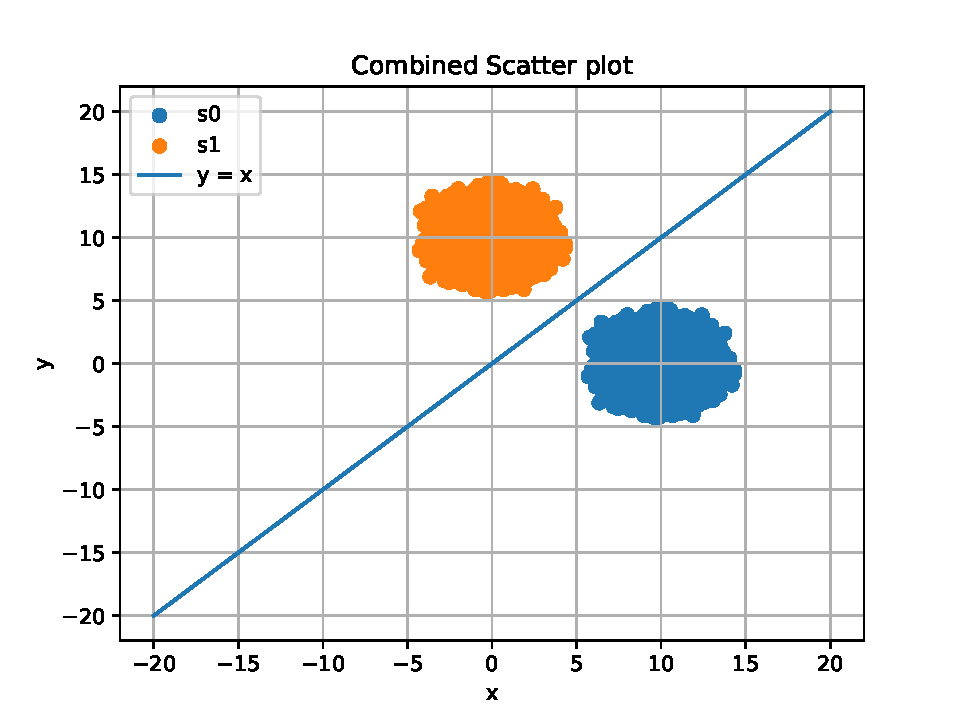
\includegraphics[width = \columnwidth]{2d.png}
\end{figure}

\newpage
\item
For the above problem, find a decision rule for detecting the symbols $\mbf{s}_0 $ and $\mbf{s}_1$.

\solution

\begin{align}
    \hat{x} &= 
    \begin{cases}
        y > x \implies s_1 \\
        y < x \implies s_0
    \end{cases}
\end{align}

%
\item
Plot 
\begin{equation} 
P_e = \pr{\hat{\mbf{x}} = \mbf{s}_1\pipe\mbf{x} = \mbf{s}_0}
\end{equation}
with respect to the SNR from 0 to 10 dB.

Program to plot the graph
\begin{lstlisting}
wget https://github.com/Abhay478/GVV_things/blob/master/code/2d_estim.py
\end{lstlisting}

\begin{lstlisting}
python3 2d_estim.py
\end{lstlisting}

\begin{figure}[!h]
    \caption{Estimation error}
    \includegraphics[width = \columnwidth]{2d_estim.png}
        \label{2d-thing}
\end{figure}
\begin{figure}[!h]
    \includegraphics[width = \columnwidth]{2d_log.png}
\end{figure}

\item
Obtain an expression for $P_e$. Verify this by comparing the theory and simulation plots on the same graph.

\solution

\begin{align}
    P_e &= \pr{\hat{\mbf{x}} = \mbf{s}_1\pipe\mbf{x} = \mbf{s}_0} \nonumber \\
    \implies P_e &= Pr(n_2 > n_1 + A) \nonumber \\
    &=  \mbf{Q}\brak{\frac{A}{\sqrt{2}}}
\end{align}

Plotted in figure ~\ref{2d-thing}

	\end{enumerate}



\end{document}